\section{Debugger Testing DSL}

\emph{DeTeL} is integrated in \ic{MPS} and interacts
with mbeddr's debugger \ic{API}. While this language is currently tightly
coupled to mbeddr, it could in theory interact with a generic debugger \ic{API}
and be implemented with a language workbench other than \ac{MPS}.
This section describes the structure of \emph{DeTeL} and the
implementation of design decisions discussed in \sect{DesignDecisions}.

\ic{DebuggerTest} is the module in which \ic{DebuggerTestcase}s and
\ic{CallStack}s are declared. 


\subsection{DebuggerTest}

\fig{fig:DebuggerTestStructure} shows the structure of \ic{DebuggerTest}: 
it \emph{contains} \ic{ITestContent}s, currently implemented by 
\ic{DebuggerTestcase} and \ic{CallStack} (described later). By
implementing this interface we can also use other concepts inside
\ic{DebuggerTest} (\hyperref[O2]{O2}). Further, \ic{DebuggerTest} refers to 
a \ic{Binary} (the compiled mbeddr program under test), \emph{imports} of other
\ic{DebuggerTest}s (enables reuse \hyperref[O1]{O1}) and an
\ic{IDebuggerBackend} that specifies the debugger backend to use
(\hyperref[M1]{M1}). Latter is implemented by \ic{GdbBackend} and allows this
way to execute debugger tests with the \ac{GDB}~\cite{gdb}.

\begin{figure}[h]
  \vspace{-2mm}
  \centering
    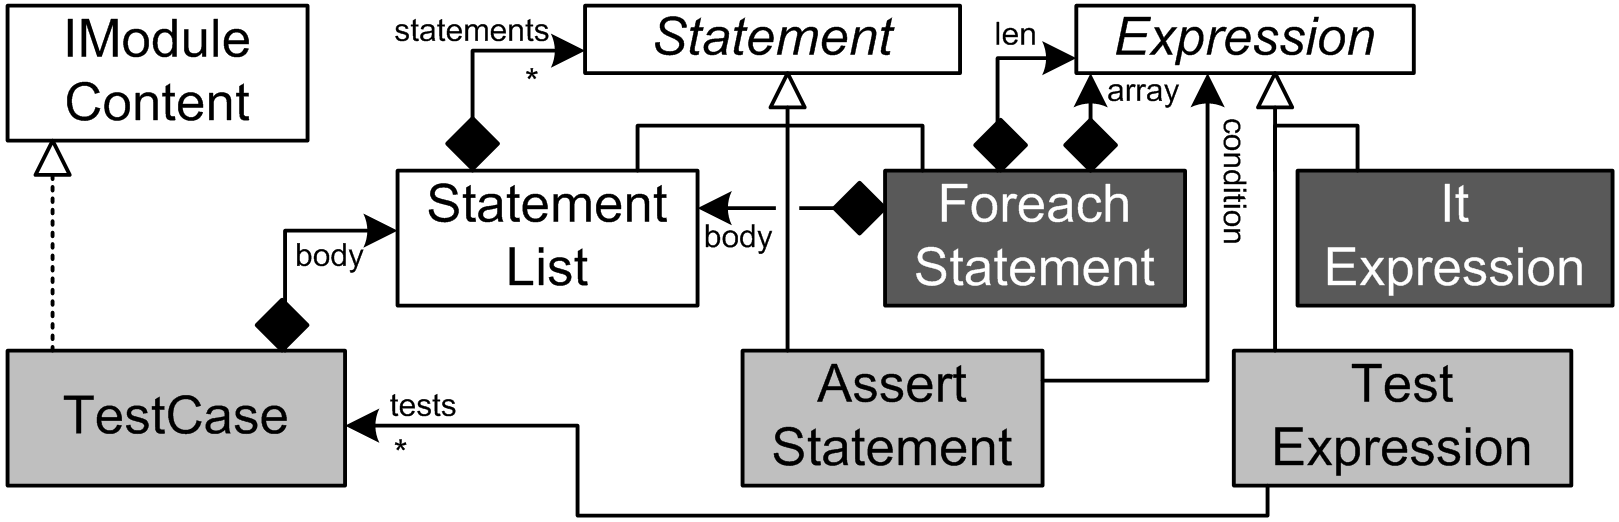
\includegraphics[width=8.5cm]{./figures/umldiag.png} 
    \vspace{-2mm}
    \caption{Structure of \ic{DebuggerTest}s}
  \label{fig:DebuggerTestStructure}
  \vspace{-2mm}
\end{figure}

\ac{MPS} comes already with the language \ic{mps.lang.test} for writing type
system and editor tests. Its \ac{MPS} integration allows users to (1) execute
tests \emph{automatically} (on the command-line and inside the \ac{IDE}) and 
(2) get the results of
executed tests visualized in a table view. All of that functionality is build
for implementations of \ic{ITestcase} - an interface from \ic{mps.lang.test}. By
implementing this interface in \ic{DebuggerTest} (our container for
\ic{DebuggerTestcase}s), we get the \ic{IDE} integration and the ability to
run our tests \emph{automatically} (\hyperref[O3]{O3}).



\subsection{CallStack}

\ic{CallStack} implements \ic{ITestContent} 
(see \fig{fig:CallStackStructure}) and is used for declaring a
stack of \ic{IStackFrame}s. Each frame specifies a \emph{name}, 
visible \emph{watches} and the \emph{location} where suspended.
We have two implementations of \ic{IStackFrame}:
\ic{StackFrame} and \ic{StackFrameExtension} 
(extends a \ic{StackFrame}).
Since a \ic{CallStack} can extend another
\ic{CallStack}, \ic{StackFrameExtension} can be used 
to specialize properties of the extended \ic{StackFrame}. Additionally, the
extending \ic{CallStack} can declare further \ic{StackFrame}s.

\begin{figure}[h]
  \vspace{-2mm}
  \centering
    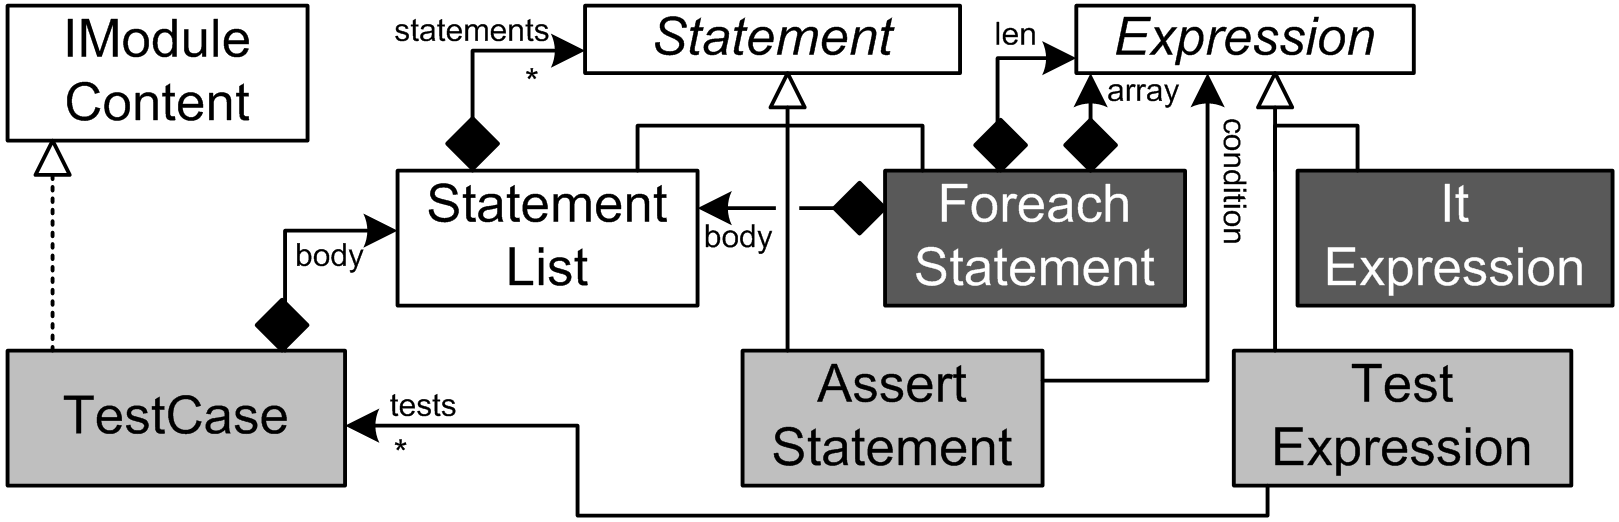
\includegraphics[width=8.5cm]{./figures/umldiag.png} 
    \vspace{-2mm}
    \caption{Structure of \ic{CallStack}s}
  \label{fig:CallStackStructure}
  \vspace{-2mm}
\end{figure}

\ic{IStackFrame} has three parts: a \emph{name} 
(\ic{IStackFrameName}), a location where suspended (\ic{ISuspendLocation}) 
and a list of visible (\ic{IWatches}).

\ic{IStackFrameName} has two implementations: \ic{Any- StackFrameName} does not
validate the name, while \ic{StackFrameName} verifies a specific
\emph{name}. Next, \ic{ISuspendLocation} with its implementations:
the location where suspended is not validated with \ic{Any- Location},
while \ic{ProgramMarkerRef} references a \ic{ProgramMarker} that represents a
specific location in an mbeddr program. Instances of \ic{ProgramMarker} do not influence
code generation, they just annotate nodes in the \ac{AST}. \ic{IWatches} is
implemented by \ic{Anywatches} and \ic{WatchesDeclaration}. First does not
validate visible watches, while the declaration specifies the \emph{name} of
watch and its value with a \ic{ValueExpression}. This expression again has two
implementors: \ic{PrimitiveValueExpression} for primitive values (\eg numbers or
characters) and \ic{ComplexValueExpression} for complex values (\eg arrays or
structs).

\subsection{DebuggerTestcase}

The structure of \ic{DebuggerTestcase} is shown in
\fig{fig:DebuggerTestcaseStructure}:
has a \emph{name}, can \emph{extend} other \ic{DebuggerTestcase}s and can be
\ic{abstract}. Further it holds the following parts:
\ic{SuspendConfig}, \ic{SteppingConfig} and
\ic{Validation- Config}. Concrete \ic{DebuggerTestcase}s require at least  
a \ic{SuspendConfig} and a \ic{ValidationConfig} (can be inherited),
while an \ic{abstract} \ic{DebuggerTestcase} requires none.
 
\begin{figure}[h]
  \vspace{-2mm}
  \centering
    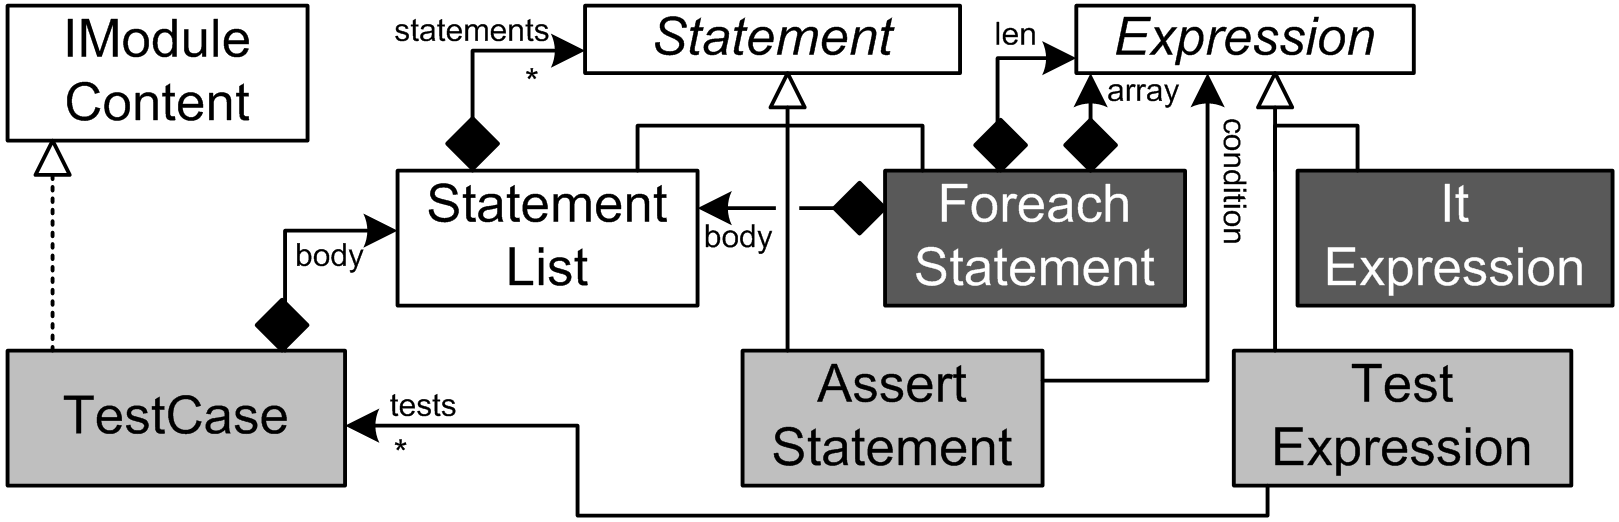
\includegraphics[width=8.5cm]{./figures/umldiag.png} 
    \vspace{-2mm}
    \caption{Structure of \ic{DebuggerTestcase}s}
  \label{fig:DebuggerTestcaseStructure}
  \vspace{-2mm}
\end{figure}

\ic{SuspendConfig} contains a \ic{ProgramMarkerRef} that points to
\emph{location} inside the mbeddr program under tests. When executing the test,
the debugger is suspended at this \emph{location}. 

\ic{SteppingConfig} is optional and contains a
list of \ic{ISteppingElement}s that are executed after suspending on
\emph{location}. This interface is implemented by 
\ic{ISteppingCommand} and \ic{SuperConfigElement}. Former is again an
interface and holds a property \emph{times} that specifies how often the command
is executed. Its implementations are \ic{StepIntoCommand},
\ic{StepOverCommand}, \ic{StepOutCommand} -- the minimal stepping commands.

\ic{ValidationConfig} contains a list of \ic{IValidationElements}. This
interface is implemented by the previously described \ic{CallStack}
and \ic{CallStackRef}, which is used for refering to a
\ic{CallStack} without having the possibility to extend it.
Finally, \ic{OnPlatform} executes contained \ic{ValidationConfig}s only if tests
are executed on the specified \ic{Platform} (possible platforms are Mac, Unix or
Windows).

\section{Testing the Debugger Extension}

The previously described debugger testing \ac{DSL} is used in this section for
testing the debugger extension of unit testing. While those
tests do not aim for full test coverage, they concentrate on the essential
scenarios to test.

Before writing tests, the program using the unit testing
language from \lst{lst:generatedUT} is annotated with markers
(see listing below). Those markers do not influence the code generation, they
are just used by \ic{DebuggerTestcases} to refer to code locations for
specifying where to suspend and for verifying where
execution suspended.

\begin{lstlisting}[language=markerDSL]
int32 main(int32 argc, string$[$ $]$ argv) {
   [return test$[$forTest$]$;] onReturnInMain
}
testcase forTest {
   [int32 sum = 0;] onSumVarDeclaration
   [assert: sum == 0;] on1stAssertInTestcase
   [int32$[$ $]$ nums = {1, 2, 3};] onNumsVarDeclaration
   for(int32_t i=0;i<3;i++) { sum += nums[i]; }
   [assert: sum == 6;] onLastStmntInTestcase
}
\end{lstlisting}	

Next, an empty \ic{DebuggerTest} \emph{UnitTesting} is created (see listing
below) that will later contain all \ic{DebuggerTestcase}s described in this
section. \emph{UnitTesting} tests against the binary
\emph{UnitTestingBinary}, which is compiled from \lst{lst:generatedUT} and further tells the
mbeddr debugger runtime to use the \emph{gdb} debugger backend.

\begin{lstlisting}[language=testingDSL]
DebuggerTest UnitTesting    tests binary: UnitTestingBinary {
                            uses debugger: gdb

}  
\end{lstlisting}

\subsection{Step Into ExecuteTestExpression}

For testing \emph{step into} on instances of \ic{Execute- TestExpression},
in the listing below a \ic{CallStack- Declaration} is created that specifies how
the stack must be organized after performing \emph{step
into} on \emph{onReturnInMain}. To reuse information and 
minimize redundance in later
\ic{DebuggerTestcase}s, two separate 
\ic{CallStack}s are created: First, \emph{inMain} 
has a single \ic{StackFrame} that expects (1) execution to be suspended at  
\emph{onReturnInMain} and (2) two watches to exist -- \emph{argc} and
\emph{argv}. Second, \emph{inTestcase} extends
\emph{inMain} by declaring on top of \emph{main} an addition
\ic{StackFrame} \emph{forTest}, which specifies no location, but two
watches: \emph{sum} and \emph{nums} (code colored
in gray is projected from the extended \ic{CallStack} and not
editable).

\begin{lstlisting}[language=testingDSL]
call stack inMain {
   0:main
      location:   onReturnInMain
      watches: {argc, argv}                     
}
   
call stack inTestcase extends inMain {
   1:forTest
      location: <any>
      watches: {sum, nums}                  
   $\gT{0}$$\gT{:}$$\gT{main}$
}
\end{lstlisting}

After declaring the \ic{CallStack}s, the listing below contains
the \ic{DebuggerTestcase} \emph{stepIntoTestcase}, which uses the declaration to
verify \emph{step into} for instances of \ic{ExecuteTestExpression}: First,
execution is suspended at \emph{onReturnInMain}, next, a single \emph{step into}
command is performed before the actual call stack is validated against
a custom \ic{CallStack} derived from \emph{inTestcase}.
This custom delcaration specializes for the \ic{StackFrame}
\emph{forTest} the expected location with \emph{onSumDeclaration}.

\begin{lstlisting}[language=testingDSL]
testcase stepIntoTestcase {            
   suspend at: 
      onReturnInMain
   then perform:                         
      step into 1 times    
   finally validate:                         
      call stack stepIntoTestcase extends inTestcase {
         $\gT{1}$$\gT{:}$$\gT{forTest}$
            overwrite location: onSumDeclaration
            $\gT{watches}$$\gT{:}$ $\gT{\{}$$\gT{sum, nums}$$\gT{\}}$
         $\gT{0}$$\gT{:}$$\gT{main}$                       
      }
}
\end{lstlisting}

\subsection{Step into/over AssertStatement}

After verifying \emph{step into} for \ic{ExecuteTestExpression}, 
\emph{step into} and \emph{over} for instances of \ic{AssertStatement} is tested
next. Since both stepping commands have the same behavior when performed at
\emph{1stAssert}, common information can be extracted into the \emph{abstract}
\ic{DebuggerTestcase} \emph{stepOnAssert} shown below: (1) execution is
suspended on \emph{1stAssert} and a custom \ic{CallStack} verifies that
execution in \emph{forTest} is (2) suspended on \emph{onArrayDecl} and
(3) watch \emph{num} has the value zero.
 
\begin{lstlisting}[language=testingDSL]
abstract testcase stepOnAssert {
   suspend at: 
      1stAssert
   finally validate:
      call stack stepOnAssert extends inTestcase {
         1:forTest
            overwrite location:   onArrayDecl
            overwrite watches: {sum=0,nums}
         0:main                      
      }
}
\end{lstlisting}

While the first \ic{DebuggerTestcase} \emph{stepIntoAssert} extending
\emph{stepOnAssert} performs a \emph{step into}, the other one
\emph{stepOverAssert} performs a \emph{step over}:

\begin{lstlisting}[language=testingDSL]
testcase stepIntoAssert extends stepOnAssert {            
   then perform:                         
      step into 1 times                            
}
testcase stepOverAssert extends stepOnAssert {            
   then perform:                         
      step over 1 times                            
}
\end{lstlisting}

\subsection{Step on last Statement in Testcase}

The last testing scenario verifies stepping on the last \ic{Statement}
(\emph{2ndAssert}) inside a \ic{Testcase} suspends execution on the calling
\ic{ExecuteTestExpression} (\emph{onReturnInMain}).
The approach for testing this scenario is similar as before:
The listing below contains the \emph{abstract} \ic{DebuggerTestcase}
\emph{steppingOnLastStmnt}, which suspends exeuction on
\emph{2ndAssert} and verifies the actual call stack has the same structure as
\emph{inMain}.

\begin{lstlisting}[language=testingDSL]
abstract testcase steppingOnLastStmnt {
   suspend at: 
      2ndAssert
   finally validate:
      call stack inMain
}
\end{lstlisting}

Next, for \emph{step over}, \emph{into} and \emph{out} a separate
\ic{DebuggerTestcase} is created, which extend \emph{steppingOnLastStmnt} and
specify the additional stepping command:

\begin{lstlisting}[language=testingDSL]
testcase stepOverLastStmnt extends steppingOnLastStmnt {            
   then perform:                         
      step over 1 times                            
}
testcase stepIntoLastStmnt extends steppingOnLastStmnt {            
   then perform:                         
      step into 1 times                            
}
testcase stepOutFromLastStmnt extends steppingOnLastStmnt {            
   then perform:                         
      step out 1 times                            
}
\end{lstlisting}		
			
	